\documentclass{article} 

\usepackage{amsmath,amsthm,amssymb,graphicx}

\graphicspath{ {C:/Users/David/SkyDrive/School/MATH 240/Assignments/} }

\newtheorem{problem}{Problem} 

\theoremstyle{definition} 

\newtheorem*{solution}{Solution} 

\begin{document} \title{Assignment 6} 

\author{Yang David Zhou, ID 260517397} 

\date{\today}

\maketitle

\begin{problem} 

Cycles and Circuits.

\end{problem}

\begin{solution}

(a) I will use the theorem proven in class that a connected simple graph is Eulerian iff it has no vertices of odd degree.\\

Take a complete graph \(G'\) with \(|V'|=11\). It has \(|E'|=\frac{|V'|(|V'|-1)}{2}\). So, \(|E'|=55\). This complete graph is Eulerian because every vertex is connected to 10 other vertices so every vertex has an even degree. Since \(G'\) is a complete graph, I can transform \(G'\) to \(G\) by removing 2 edges. \\

So I remove the 1st edge, say the edge was \((u,v)\). Now both \(u\) and \(v\) have an odd degree of 9. I must remove a 2nd edge. I either remove an edge that is adjacent to \(u\) or \(v\), or I remove an edge not adjacent to \(u\) or \(v\) to achieve \(G\).\\

In the case where I must remove an edge \((v,w)\) that is adjacent to \(v\), I now have vertices \(u\) and \(w\) that have an odd degree of 9. \(|E'|=53\) but the graph is not Eulerian. The case for an edge adjacent to \(u\) is symmetrical.\\

In the case where I must remove an edge \(w_i,w_j\) that is not adjacent to either \(u\) or \(v\), I now have 4 vertices, \(u\), \(v\), \(w_i\), and \(w_j\) that have an odd degree of 9. Again, \(|E'|=53\) but the graph is not Eulerian. \\

Thus \(G\) cannot be Eulerian. \\

(b) The idea here is similar to that in (a). A complete graph \(G'\) with \(|V'|=11\) has a Hamiltonian Cycle because starting from any vertex, there is always an edge to any other unvisited vertex.\\

To get from \(G'\) to \(G\), I must remove 2 edges. Either I remove 2 non-cycle edges or I remove at most 2 cycle edges.\\

In the case where I must remove 2 non-cycle edges, the original Hamiltonian Cycle from \(G'\) is still a Hamiltonian Cycle in \(G\) so \(G\) is a Hamiltonian Graph.\\

In the case where I must remove 2 cycle edges, there are two options. Either I removed two edges that share an endpoint vertex or I removed two edges that do not. 

If I removed two edges \((u_i,v)\) and \((v,u_j)\) then I can rebuild the Hamiltonian cycle by removing some non-adjacent edge \((u_k,u_l)\) and adding \((u_i,u_j)\), \((v,u_k)\) and \((v,u_l\), all of which exist because they were not the edges removed from the complete graph \(G'\). This graph contains a Hamiltonian cycle.

If I removed two edges \((u_i,v_i)\) and \((u_j,v_i)\) such that a path still exists on the cycle from \(v_i\) to \(u_j\) then I can rebuild the Hamiltonian cycle by adding \((u_i,u_j)\) and \((v_i,v_j)\). This graph contains a Hamiltonian cycle. \\

Thus \(G\) must be Hamiltonian.

\end{solution}

\begin{problem} 

Trees.

\end{problem}

\begin{solution}

For this problem I assume that a path consists of edges and the vertices they connect so two paths intersect if they share at least one vertex, but not necessarily any edges.\\

Proof by induction.\\

In a tree of consisting of 1 node, the longest "path" is the single node. So the two longest paths must intersect the single node.\\

I assume that the two longest paths must intersect on a tree \(T'\) of \(n\) nodes.\\

I can take a tree \(T\) with \(n+1\) nodes and remove a leaf node to create \(T'\).\\

I assumed that in \(T'\) the two longest paths must intersect.\\

In order to get back to \(T\), I must add back the node I removed. So I either add a child node to a leaf node or I add a leaf node to a parent node.\\

If I add another leaf node \(v\) to an existing parent node \(u\), the new set of maximum length paths might include a path that begins at \(v\) if the children of \(u\) were leaf nodes that were in the set of maximum length paths. All the previous maximum length paths passed through \(u\) and the new maximum length path that begins at \(v\) also passes through \(u\). So all the maximum length paths intersect at \(u\). If the new set of maximum length paths do not include a path through \(v\) then the maximum length paths in \(T\) are identical as in \(T'\).\\

If I add a child node \(v\) to an existing leaf node \(u\), the diameter of \(T\) may or may not increase from that of \(T'\). If it does increase, then all the new maximum length paths must include \(v\) so all new maximum length paths must intersect at least at \(v\) and \(u\). If the diameter does not increase then the maximum length paths in \(T\) are identical as in \(T'\).

\end{solution}

\begin{problem} 

Joyal Codes.

\end{problem}

\begin{solution}

(a) 

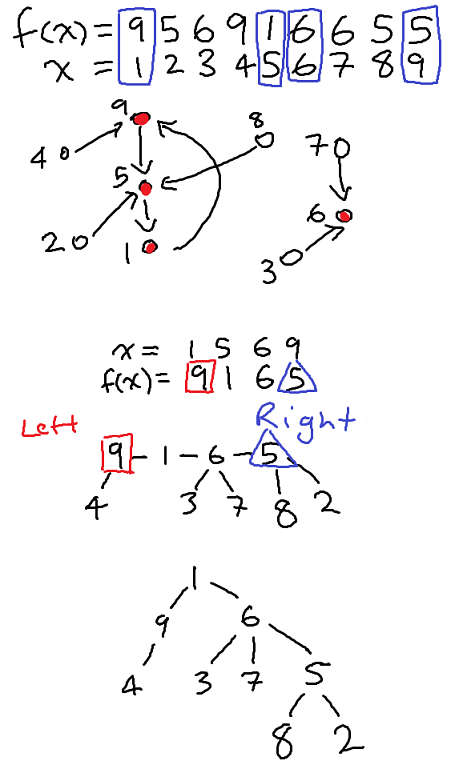
\includegraphics[scale=1]{a6q3a} \\

(b) The path from left to right is 4852 which I add to the table in order, \\

\begin{tabular}{lllll}
f(x) & 4 & 8 & 5 & 2 \\
x    & 2 & 4 & 5 & 8
\end{tabular}\\

And then I add the remaining nodes, \\

\begin{tabular}{llllllllll}
f(x) & 8 & 4 & 5 & 8 & 5 & 4 & 2 & 2 & 4 \\
x    & 1 & 2 & 3 & 4 & 5 & 6 & 7 & 8 & 9
\end{tabular} \\

So the code is 845854224.

\end{solution}

\end{document}